\documentclass{article}
\usepackage[utf8]{inputenc}
\usepackage{todonotes}
\usepackage{natbib}
\usepackage{graphicx}
\usepackage{wrapfig}
\usepackage{depreequantum}
\usepackage[]{acronym}
\usepackage{hyperref}

\title{Einführung in die Raumfahrt zusammenfassung}
\author{Magnus Offermanns}
\date{Fall 2019}



\begin{document}

\maketitle
\tableofcontents
\section{Acronyms}
\begin{acronym}
\acro{s/c}{Spacecraft}
\acro{s/w}{Software}
\acro{h/w}{Hardware}
\acro{EOL}{End of Life}
\acro{Eng}{Engineering}
\acro{Sys}{System}
\acro{Comm}{Communication}
\acro{GNC}{Guidance, Navigation and Control}
\acro{ADCS}{Attitude Determination \& Control Subsystem}
\acro{AIV}{Assembly, Integration and Verification}
\acro{OBDH}{On Board Data Handling}
\acro{MO}{Mission Operation}
\acro{DA}{Data Analysis}
\acro{LEO}{Lower Earth orbit}
\acro{GEO}{Geosyncronouse Orbit}
\acro{GTO}{Geostationary Transfer Orbit}
\acro{WSB}{Weak Stability Boundary}
\acro{RTG}{Radio-Thermonukleid Generator}
\acro{AU}{Astronomical Unit}
\acro{LHB}{Late Heavy bombardment}
\end{acronym}

\section{rFirst set of Slides,Our Solar System}
\subsection{Origin of a solarsystem}
In the first stage of galaxy building the matter that will later be our galaxy is a Protosolar fog with a huge diameter of 20000 \ac{AU}. \ac{AU} is the distance between the earth and the sun. After some time the fog collapsed under its own gravitational pull resulting in an increase in density. We call this stage protoplanetary disk with an diameter of about 200 \ac{AU}. Over time the dust formed to bigger and bigger chuncks due to gravity. So the planets were formed.\\ The cause why the terrestrial planets formed closer to the sun was that the temperature at the inner planets (Mercury, Venus, Earth, and Mars)) was to high to keep volantile molekules to them. Just heavy atoms like iron, nickel, and aluminum. The outer planets (Jupiter, Saturn, Uranus, and Neptune) were able to collect more volantile molekules resulting in much bigger size. The last stage that we encoutered was the \ac{LHB} which is a time in which the moon and the earth was hit by a lot of Meteors.

\subsection{Geography of our Solar system}
A picture of our solar system can be found in figure \ref{fig:Foliensatz1:geography}. Ein Merksatz für unser Sonnensystem ist: Unser Vater erklärt mir jeden Sonntag unsere neun planeten. While we only have eight planets. Pluto is a Dwarf planet
\begin{figure}
    \centering
    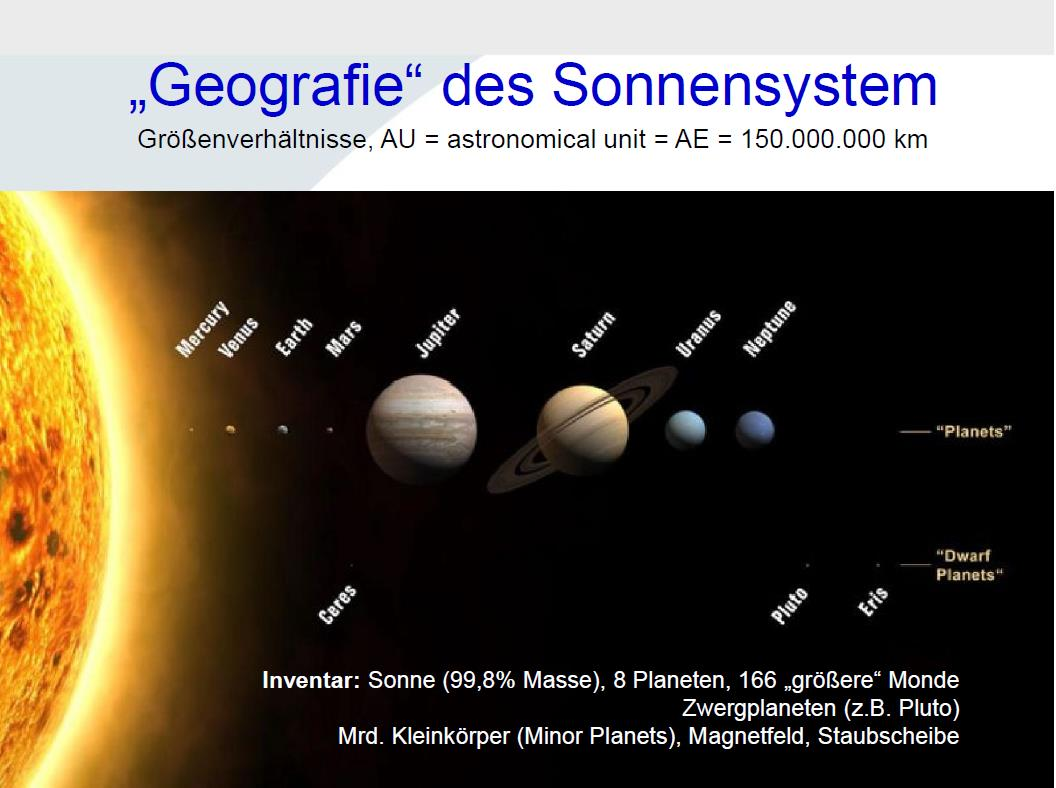
\includegraphics[width=0.7\textwidth]{images/Foliensatz1_geography_of_our_solarsystem.png}
    \caption{A picture of our Solarsystem}
    \label{fig:Foliensatz1:geography}
\end{figure}

\subsection{Definitons}
\subsubsection{What is a Planet}
A celestial body is a planet if it fullfills the following points:
\begin{enumerate}
    \item If it orbits around the sun\\
    \item It needs suffiecient mass for its self-gravity to overcome rigid body forces so that it asumes hydrostatic equilibrium (almost round shape)
    \item Hast cleared its neighbourhood from debre and other foreign bodies
\end{enumerate}
\subsubsection{What is a dwarf planet}
A Dwarf Planet is a new class of Celestial body of which pluto is the prime example. In comparison to a planet it can still have trash and other objects in it orbit that means a Dwarf planet is a dwarf planet if it fullfills the following points:
\begin{enumerate}
    \item If it orbits around the sun\\
    \item It needs suffiecient mass for its self-gravity to overcome rigid body forces so that it asumes hydrostatic equilibrium (almost round shape)
    \item Has not cleared its neighbourhood from debre and other trash yet
    \item and it needs to not be a Satellite
 \end{enumerate}   
\subsubsection{Small Solar-system Bodies}
Are all other bodies orbiting the sun except satellites

\subsubsection{Other celestial bodies that need to be distinguised}
\begin{enumerate}
    \item  Komet\\
    A big pile of rock orbiting the sun.
    \item Asteroid\\
    smaller pile of rock that orbits the sun
    \item Meteroride\\
    Even smaller object flying through space orbiting the sun. The size is between meters and $\mu$ meters.
    \item Meteor\\
    A Meteoride hitting earth but burning up in the athmosphere
    \item Meterorite\\
     A meteor that hits Earth without burning up in the atmosphere
\end{enumerate}

\subsubsection{The interplanetary medium}
It consists of the following particles. First dust, cosmic rays from \ac{SN}, \ac{BH} and neutron-stars. Additonally there are magnetic fields and Sunwinds.

\subsection{The scattered disk}
The scattered disk is assortment of millions of comets with different rings. The innermost being the Kuiper Nelt. It is thought that this might be the cause for the amount of regular comets we see. The comets have a broad band with of eccentricities and inclination. The whole Comet belt is called the Oort Cloud and is a cloud around our solar system.





\section{Second sets of Slides, Basics Raumfahrtsysteme}
\subsection{Raumfahrt agenturen}
\begin{enumerate}
    \item European space agency\\
    Ausschliesslich friedliches Mandat. 5.6 Mrd Jahres ettat. Berühmet Projekte zb: Galieo, Rosetta
    \item NASA \\
    mitlitärische und Zivile Forschung. Nationale behörde Präsident setzt administrator ein\\ 4 Direktorate, Aeronautik, Exploration Systems, Science, Space Operations
\end{enumerate}
\subsection{Wie entsteht eine mission}
Erster schritt ist das brainstorming: Call for ideas than from all proposed ideas one mission is preliminaryly selected. Than a mission definition is written, \ac{AO}, vorläufige \ac{p/l} selection, than phase 0 is completed -> phase 0 is the work to do before the project can start. Lastly requirements are defined that the projet should fullfill (Lastenheft).
\\\\
Than a political OK is given with the dedication of funding. all prime contractors and subcontractors are defined and the requirements for them is done as well.
\subsubsection{What are the parts \ac{s/c} consists of?}
\begin{enumerate}
    \item Astronautis/Science
    \item \ac{Sys} Engineering
    \item \ac{Comm}\\
    Communication with spacecrafts in space
    \item \ac{OBDH}\\
    How is the data displayed in the spacecraft. What is send home.
    \item \ac{s/w} \ac{Eng}
    \item Electrical/Power\\
    Electrical wiring, power generation $\cdots$
    \item propulsion\\
    What and how do we burn stuff to get into space
    \item \ac{ADCS}\ac{GNC}
    Monitoring and controll of Orientation of spacecraft and Navigation in relation to the earth (where are we in space)
    \item Thermal\\
    Overheating prevention in space. Prevention of burning up at reentry
    \item Mechanical \\
    Mechanical stuff
    \item Crew\\
    Training of Crew
\end{enumerate}

What else needs to be though of when designing a mission:
\begin{enumerate}
\item Testing\\
 Testing of hardware: testing of hardware
\item \ac{AIV}\\
Assembly of hardware and the intense testing that follows.
\item{Launch}\\
Launching spacecrafts into space
\item Operations\\
 Is the means necessary to run a robot, spacecraft during the mission a.e. the guys currently controling the mars rover
 \item Disposal\\
  Where does the stuff go which we leave in space, i.e. Satellite disposal after \ac{EOL}
\end{enumerate}

\subsection{Mission life cycle}
 Every mission has multiple predefined phases. Starting with Phase 0 and ending with Phase F. 
 \begin{enumerate}
     \item \textbf{Pre-phase A} Conceptual study\\
     
     \item \textbf{Phase A} Preliminary analysis\\
      
      \item \textbf{Phase B}  Definition\\
      Defining the requirements of all systems. Review of the proposed desings. Non-Advaocate review i.e external review
      \item \textbf{Phase C/D} Design \& Development \\
      Preliminary Desing review -> check of first design proposal and improvement. Critical Design review -> Reveiw of the things that will be build right after this step. Test Readinesss Review -> is the hardware done so that all tests can start. Flight readyness review -> test if the hardware is ready to fly
      \item \textbf{Phase E} Operation phase \ac{MO} \& \ac{DA}\\
      Running the mission and the extended mission if all mission goals of the primary mission are complete
      \item \textbf{Phase F} Disposal\\
      How do we get rid of our hardware in space 
      
 \end{enumerate}

\subsection{Basics of Orbital mechanics}

\subsubsection{Conic Sections}
There are four kinds of conic sections which are used to shoot satelites into space. THey are generated by cutting through the cone. The cut itself than has different forms. They are defined by their \textbf{eccentricity}.\\\\
\textbf{The eccentricity is the distance between the two focal points divided by the length of the major axis}\\
\\
The focal points are the two points from which the summed up distance is always constant i.e d(\ac{s/c},$f_1$)+d(\ac{s/c},$f_2$)=constant. The major axis is the longer side of the two sides of the conic section a.e. the longer side of the elipse. The shorter side is called minor axis.\\
\\
\begin{wrapfigure}{r}{5cm}
\centering
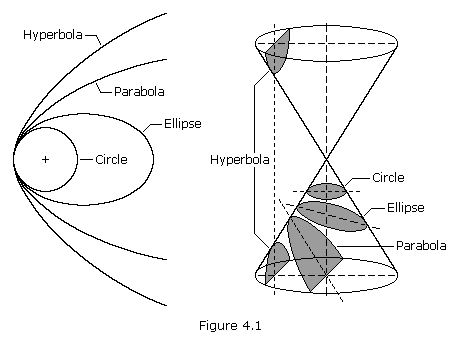
\includegraphics[width=0.4\textwidth]{images/Foliensatz2_conecut.png}
\end{wrapfigure}
There are four different cases the first beeing the circle with eccentricity 0 because the focal points touch. The use case is a geostatic satelite. The second case is the elipse where the eccentricity is greater than 0 but smaller than 1. Such a orbit would be usefull for all spacecrafts that should come back to earth. The third case is the special case in which the eccentricity is 1 which is called parabola. The two arms of the parabola get parallel in infinity. Such a cut is achieved when we cut the cone in parallel to its surface. A usecase for the parabola is a into the galaxy traveling spacecraft for example voyager. The last conic cut is Hyperbola wich is a cut in the right angle to the ground plane. The arms of the hyperbola are extending more and more and do not get parallel. This is also a trajectory for a outbound \ac{s/c}.

\begin{table}[h]
\begin{tabular}{|l|l|l|l|}
\hline
\textbf{Conic Section} & \textbf{Eccentricity,e}   & \textbf{(Major axis)/2}    & \textbf{Energy} \\ \hline
Circle                 & 0                         & =radius                    & \textless{}0    \\ \hline
Ellipse                & 0\textless{}e\textless{}1 & \textgreater{}0 (positive) & \textless{}0    \\ \hline
Parabola               & 1                         & infinity                   & 0               \\ \hline
Hyperbola              & \textgreater{}1           & \textless{}0 (negative)    & \textgreater{}0 \\ \hline
\end{tabular}
\end{table}

\subsubsection{Grundlagen Orbitalmechanik}
To mathematically describe an orbit one must define six quantities.
In the first step we define the elipse on which the space craft lies independent of its pose in 3d space. Therefore we need the first two items of the enumerate \ref{enum:Foliensatz1:Grundlagen_Orbitalmechanik} below. The semi major axis is the major axis/2 together with the Eccentricity we can calculate the minor axis and the form of the Cone cut.\\ The next thing we need is the inclination which describes the angle between a plane through the equator and the actual plane that the orbit lies on. So this parameter is the first parameter that describes the orbit in 3D. To explain the next parameter we first have to describe what the Periapsis is. It is the point which is closest to the object that is orbited (primary, planet, sun ...) the opposite i.e. the point furthest away from the object that is orbited is Apoapsis. Additionally we need to describe what the Ascending node and the descending node are. We can imagine that we still need a angle of the orbit which we denote as i (inclination)=0. As a point of reference we take the Frühlingsstern also known as 1st point of ares. An ellipse that would pass through a plane which is described by a vector in the right angle to the vector that goes from the first point of Aries to the object that we are orbiting would have inclination 0. Now the point at which the satellite that lies on our inclined orbit passes the plane through the 1st point of Aries upwards is the ascending node. The point at which the satellite crosses the line to go below it is called descending node. This describes in which direction the satellite is flying. Now the Longitude of the ascending node is the angle from the point of Aries to the ascending node if our orbit would have inclination 0. The argument of Periapsis w is the angle from the ascending node to the vector from the orbiting object to the Periapsis. The last paramter is the time of the periapsis passage T. It is the time when the satellite crosses the periapsis and serves as orientation point. The only thing that is missing here is the frequency of passing but who cares (maybe add it later) 
\begin{enumerate}
\label{enum:Foliensatz1:Grundlagen_Orbitalmechanik}
    \item Semi-Major Axis,a
    \item Eccentricity,e
    \item Inclination, i
    \item Longitude of Ascending Node,$\Omega$
    \item Argument of Periapsis w
    \item Time of Periapsis Passage, T
\end{enumerate}

\subsubsection{Orbits}
There are multiple special orbits used for different purposes. The first class of special orbits are \textbf{Geosynchronouse } orbits. This orbits have the same frequency around the earth as the earth. That means that they return to the same place in the sky every day.\\A special case of \textbf{Geosynchronouse} are the \textbf{geostationary} orbits where the satellite rotates at the same speed as the earth at the equator having a inclination \textbf{i} and eccentricity \textbf{e} of 0. The result is that the satellite stays fixed in the night sky. If someone wants to receive a signal from this kind of satellites the satellite dish does not need to be moved. Examples are TV satellites.
\todo{slides 24 till 29 how do we calculate the stuff there}

\subsection{Transferstrategies in the Solarsystem}

\subsubsection{Hohmann Transfer}
\begin{wrapfigure}{r}{5cm}
\centering
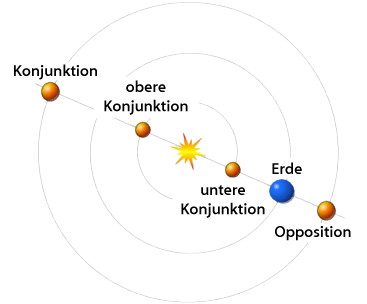
\includegraphics[width=0.3\textwidth]{images/Foliensatz2_konjunktion.png}
\caption{A conjunktion in 3d Space}
\label{img:Foliensatz1:conjunktion}
\end{wrapfigure}
Is usefull because it needs the minimum amount of energy to reach the goal. That means of course that we do not need that much fuel. The environment needs that both the start (earth) and the goal (a.e Mars) are in conjunction.\\ What does conjunction mean: It means from earth it means that the two stars touch in the nightsky. In 3d this can be seen in figure \ref{img:Foliensatz1:conjunktion}.

\subsubsection{Belbruno transfer}
The Belbruno transfer uses Lagrange points in the solar system to navigate through space without the use of $\delta v$. The advantage is the almost non existing energy a disadvantage is that the time to reach anything is very long -> a.e. to reach mars for ever. Examples for the use of the \ac{WSB} is the Hiten-Lunarlander. Another interesting mission would be to reach the Galilean moons through the Lagrange point 1 of Earth and Sun.

\subsubsection{Trajectories}
There are 3 orbits that are of importance. First beeing the \ac{LEO} being the orbit in which MIR and the ISS fly. The \ac{LEO} has a disadvantage of beeing far away the Signal takes 0.25 seconds back and forth which makes it to far away for real time applications. The second one is the \ac{GEO} the geostationary orbit. The last one is the \ac{GTO} it is a Hohmann transfer orbit from which it is the most energy saving to go from one eliptial orbit into another one. \\\\ For trajectories there are four different kinds similar to the orbits described in \ref{}. First is the Eliptical orbit which uses the mininmal energy. It can also be used for swing by maneuvers \ref{}. The second is a parabolic curve the apoapsis is at infinity the necessary $\Delta v$ needed to get to this orbit is called Entweichgeschwindigkeit. The last orbit is called a Hyperbolic orbit it is parabolic and also flys away from earth but has additional $\Delta v$. The last way to get away from our planet is usage of a Belbruno/low energy transfer transfer \todo{was ist ein belbruno transfer}(
\href{https://en.wikipedia.org/wiki/Low-energy_transfer}{Wikipedia page low energy transfer}) 

\subsubsection{Aerobreaking and Aero capture}
Aerobreaking is the deceleration using the atmosphere of a planet. This is usefull if to much $\delta v$ is is left in order to land on the surface of another planet. Therefore the trajectory gets changed into a elliptical orbit around the goal planet. At every flyby the \ac{s/c} is dipping into the atmosphere and gets decelerated by the air resistance. If the \ac{s/c} is decelerated enough the landing or constant orbiting can start.\\Aerocapture is a maneuver in which the aerobreaking happens in one surrounding of the goal planet instead of multiple. For aerobreaking the composition of the athmosphere needs to be very well known because we decelerate very close to the heat maximum while at aerobreaking the deceleration happens much less aggressive.

\subsection{Communication}
In communication in space distances are so far that signals travel very long (a.e. Mars 13 minutes). This is just one of the minor challenges of space travel. Normally radiowaves are send out in a bowl (Omnidirectional) this would mean that a lot of power wouold be lost. Therefor highly directional high gain antennas are used for communication. But the antennas need to be orientated towards each other.\\\\ The main communicator is the \textbf{NASA Deep Space Network} with 3 stations in Goldstone (USA), Madrid and Canberra which can cover the whole space at all time. Unfortunately the resources are running out and the \textbf{NASA Deep Space Network} has to support more and more Missions. Another tracking system is the \textbf{ESA-ESTRACK} with 9+3 stations world wide. The center is the \textbf{ESOC (Europ.
Space Operations Center,
Darmstadt)}

\subsection{Energysupply in space}
\subsubsection{Solar cells}
Solar cells are a sustainable source of power in missions close to the sun(Voyager is to far away). THe maximum distance is Jupiter. They use Gallium Arsenid because it degrades slower than silicone.  Sometimes the power needs to be reduced because the cooling is harder in space.
\subsubsection{\ac{RTG}}
\ref{fig:Foliensatz1:RTG} 
\begin{wrapfigure}{r}{6cm}
    \centering
    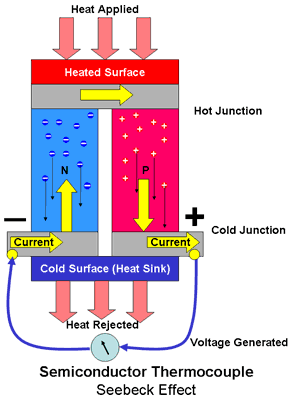
\includegraphics[width=0.3\textwidth]{images/Foliensatz2_RTG.png}
    \caption{The setup of a \ac{RTG}}
    \label{fig:Foliensatz1:RTG}
\end{wrapfigure}
A \ac{RTG} uses a Radioactive Plutonium-pellet and the Seebeck effect to generate power. It is the source for deepspace missions as Pioneer 10 \& 11, Voyager 1 \& 2 and so on.\\
\\
The seebeck effect is working with temperature differences. One side is cooled one side is heated. two conductors touch both the cold and the warm side. This results in a temperature difference. The setup is displayed in figure 


\section{Das Sonnensystem}
\subsection{Entstehung}

Abstände der Planeten

\end{document}